\documentclass[border=10pt]{standalone}

\usepackage{tikz}
\usepackage{tikzsymbols}
\usetikzlibrary{calc,patterns,shapes.geometric}

\def\centerarc[#1](#2)(#3:#4:#5){\draw[#1] ($(#2)+({#5*cos(#3)},{#5*sin(#3)})$) arc (#3:#4:#5);}

\begin{document}
	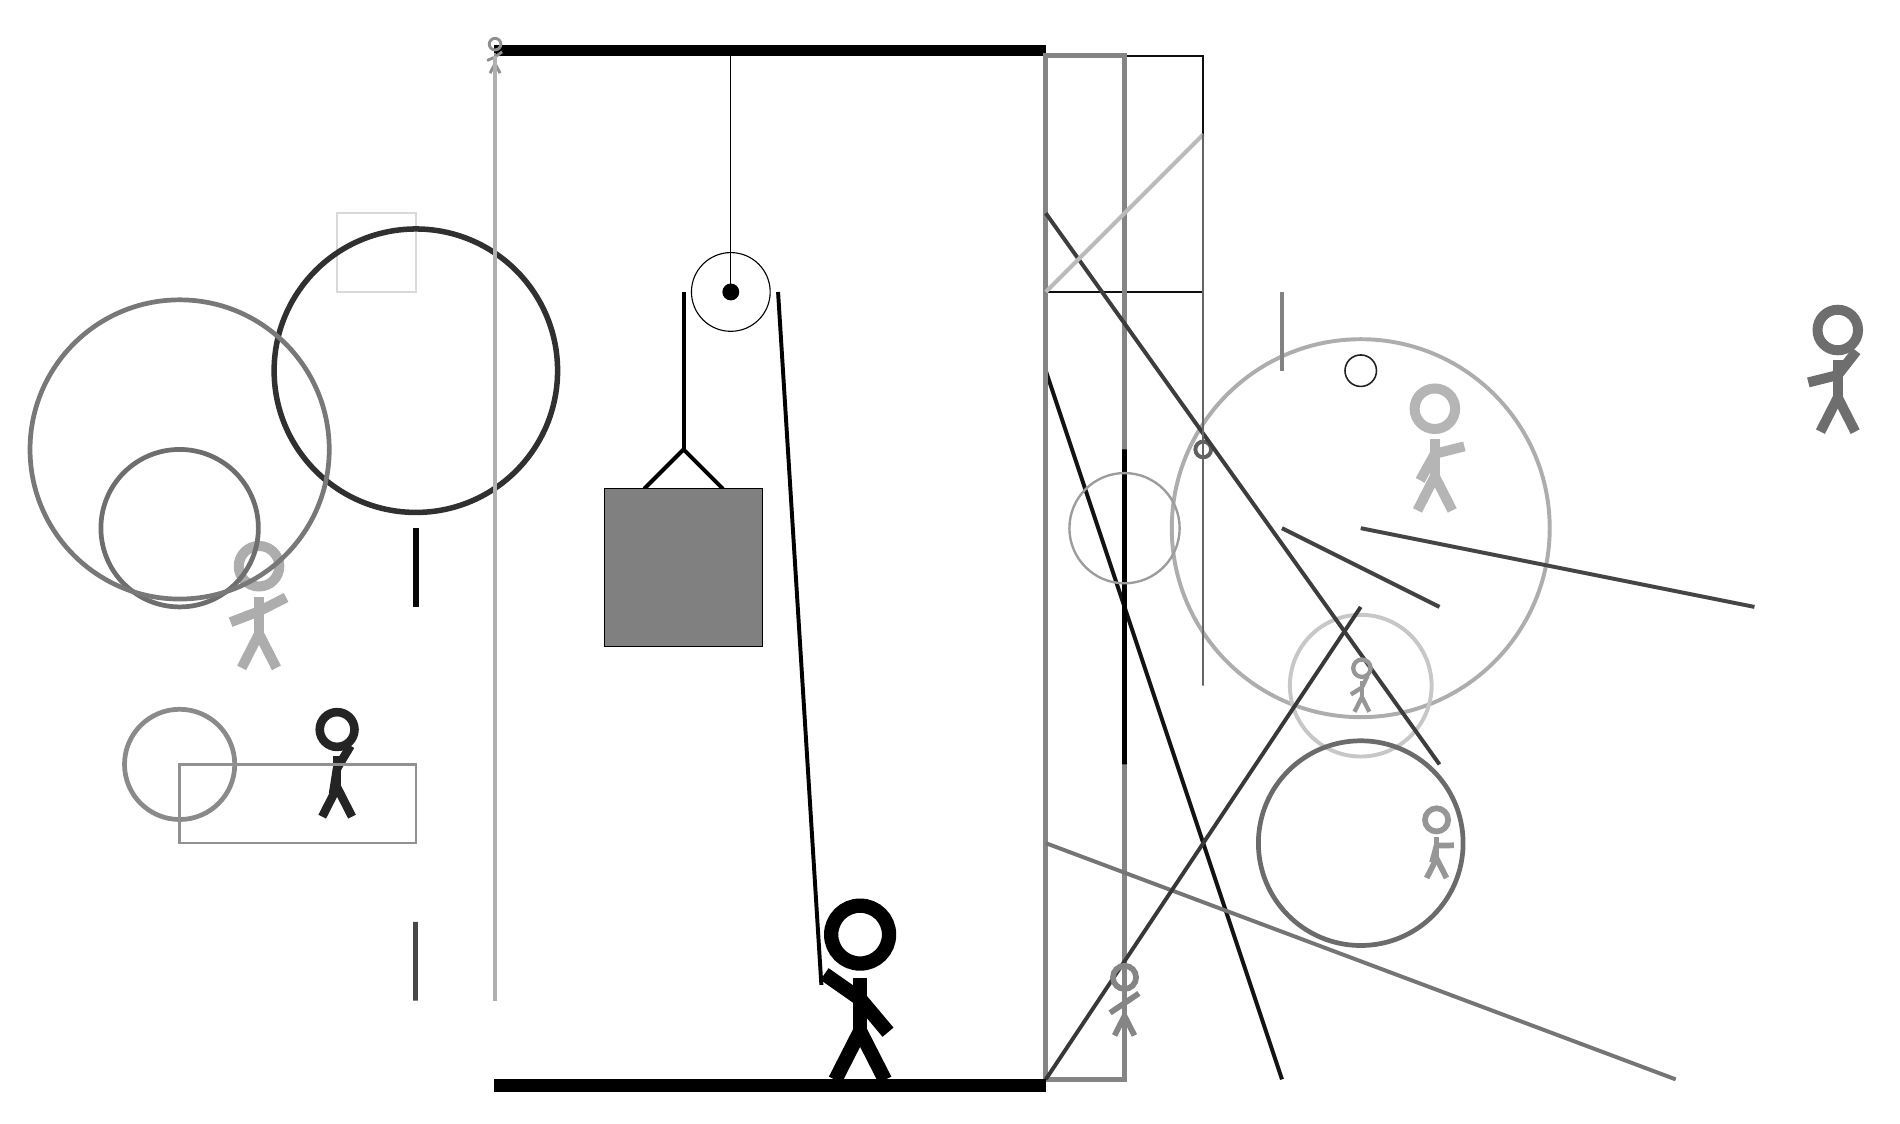
\begin{tikzpicture}
		%%%%% START %%%%%
		
		\draw[fill=black] (-2, 10) rectangle (5, 10.125);
		
		\draw (1, 7) circle (0.5);
		\draw[fill=black] (1, 7) circle (0.1);
		\draw (1, 10) -- (1, 7);
		
		\node[line width=0.2mm, color=black!86] at (-4, 1) {\Strichmaxerl[6][81][59]};
		
		\node[line width=0.6mm, color=black!44] at (-2, 10) {\Strichmaxerl[2][24][36]};
		\node[line width=0.7mm, color=black!57] at (15, 6) {\Strichmaxerl[7][14][52]};
		\draw[line width=0.5mm, color=black!74](10, 3) -- (8, 4);
		\node[line width=0.2mm, color=black!41] at (10, 0) {\Strichmaxerl[4][75][1]};
		
		\draw[line width=0.7mm, color=black!97] (-3, 3) rectangle (-3, 4);
		
		\draw[line width=0.3mm, color=black!15] (-4, 7) rectangle (-3, 8);
		\draw [line width=0.7mm, color=black!81](-3, 6) circle (1.8);
		\draw [line width=0.5mm, color=black!32](9, 4) circle (2.4);
		\draw [line width=0.5mm, color=black!62](7, 5) circle (0.1);
		
		\draw[line width=0.5mm, color=black!93](5, 6) -- (8, -3);
		
		\draw[line width=0.3mm, color=black!94] (5, 10) rectangle (7, 7);
		\draw[line width=0.6mm, color=black!48] (6, 10) rectangle (5, -3);
		\draw [line width=0.5mm, color=black!22](9, 2) circle (0.9);
		\draw[line width=0.6mm, color=black!100] (6, 1) rectangle (6, 5);
		\draw [line width=0.2mm, color=black!87](9, 6) circle (0.2);
		
		\draw [line width=0.6mm, color=black!46](-6, 1) circle (0.7);
		\draw[line width=0.5mm, color=black!54](5, 0) -- (13, -3);
		\draw[line width=0.5mm, color=black!31](-2, -2) -- (-2, 10);
		
		\draw[line width=0.5mm, color=black!78](5, -3) -- (9, 3);
		\draw[line width=0.5mm, color=black!76](5, 8) -- (10, 1);
		
		\node[line width=0.7mm, color=black!32] at (-5, 3) {\Strichmaxerl[7][21][27]};
		
		\draw[line width=0.5mm, color=black!27](5, 7) -- (7, 9);
		\draw[line width=0.5mm, color=black!73](9, 4) -- (14, 3);
		\draw[line width=0.3mm, color=black!60] (7, 9) rectangle (7, 2);
		
		\draw[line width=0.6mm, color=black!72] (-3, -2) rectangle (-3, -1);
		
		\draw [line width=0.6mm, color=black!58](9, 0) circle (1.3);
		\node[line width=0.2mm, color=black!29] at (10, 5) {\Strichmaxerl[7][61][14]};
		\node[line width=0.6mm, color=black!48] at (6, -2) {\Strichmaxerl[4][34][34]};
		\node[line width=0.3mm, color=black!41] at (9, 2) {\Strichmaxerl[3][32][64]};
		\draw [line width=0.3mm, color=black!39](6, 4) circle (0.7);
		
		\draw [line width=0.6mm, color=black!57](-6, 4) circle (1.0);
		\draw[line width=0.5mm, color=black!49](8, 7) -- (8, 6);
		\draw [line width=0.6mm, color=black!53](-6, 5) circle (1.9);
		\draw[line width=0.3mm, color=black!43] (-3, 1) rectangle (-6, 0);
		
		\draw[line width=0.5mm] (-0.1, 4.5) -- (0.4, 5.0) -- (0.9, 4.5);
		\draw[fill=black!50] (-0.6, 4.5) rectangle (1.4, 2.5);
		
		\draw[line width=0.5mm] (0.4, 7) -- (0.4, 5.0);
		\centerarc[line width=0.5mm](1, 7)(0:180:0.6);
		\draw[line width=0.5mm](1.6, 7) -- (2.15, -1.8);
		
		\node at (2.6, -1.9) {\Strichmaxerl[10][-35][-50]};
		
		\draw[fill=black] (-2, -3) rectangle (5, -3.15);
		
		%%%%% END %%%%%
	\end{tikzpicture}
\end{document}